\iffalse
\documentclass[journal,10pt,twocolumn]{article}
\usepackage{graphicx}
\usepackage[margin=0.5in]{geometry}
\usepackage[cmex10]{amsmath}
\usepackage{array}
\usepackage{booktabs}
\usepackage{listings}
\title{\textbf{Line Assignment}}
\author{Bhavani Kanike}
\date{October 2022}

\providecommand{\norm}[1]{\left\lVert#1\right\rVert}
\providecommand{\abs}[1]{\left\vert#1\right\vert}
\let\vec\mathbf
\newcommand{\myvec}[1]{\ensuremath{\begin{pmatrix}#1\end{pmatrix}}}
\newcommand{\mydet}[1]{\ensuremath{\begin{vmatrix}#1\end{vmatrix}}}
\providecommand{\brak}[1]{\ensuremath{\left(#1\right)}}

\begin{document}

\maketitle
\paragraph{\textit{Problem Statement} 
\fi
ABCD is a quadrilateral in which $\vec{P}, \vec{Q}, \vec{R}$ and $\vec{S}$ are mid-points of the sides AB, BC, CD and DA (see Fig \ref{fig:9/8/2/1}). AC is a diagonal. 
		
Show that 
\begin{enumerate}
	\item $SR \parallel AC$ and $SR =\frac{1}{2} AC$
\item $PQ = SR$
\item $PQRS$ is a parallelogram.
\end{enumerate}
 	\begin{figure}
		\centering
 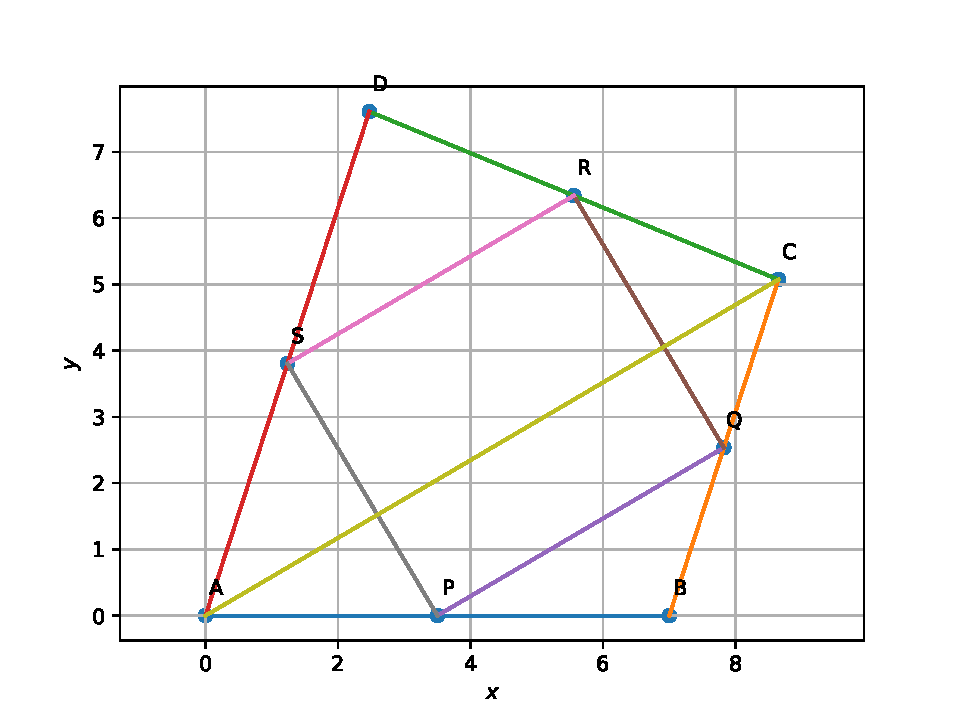
\includegraphics[width=\columnwidth]{chapters/9/8/2/1/figs/line1.pdf}
		\caption{}
		\label{fig:9/8/2/1}
  	\end{figure}
	\solution 
	Using 
	  \eqref{eq:section_formula},
	\begin{align}
		\label{eq:9/8/2/1}
		\begin{split}
		\vec{P} &= \frac{\vec{A}+\vec{B}}{2}\\
 \vec{Q} &= \frac{\vec{C}+\vec{B}}{2}\\
 \vec{R} &= \frac{\vec{C}+\vec{D}}{2}\\
 \vec{S} &= \frac{\vec{D}+\vec{A}}{2}
		\end{split}
	\end{align}
\begin{enumerate}
	\item
	Consequently, 
	\begin{align}
\vec{R}
		-\vec{S} &= \frac{\vec{C}-\vec{A}}{2}
		\\
		\implies SR &\parallel AC
	\end{align}
	Also, 
	\begin{align}
		\norm{\vec{R}
		-\vec{S}} &= \frac{\norm{\vec{C}-\vec{A}}}{2}
		\\
		\implies SR &= \frac{1}{2}AC
	\end{align}
\item 	From 
		\eqref{eq:9/8/2/1},
	\begin{align}
\vec{R}
		-\vec{S} = \vec{Q}-\vec{P}
	\end{align}
	which means that $PQRS$ is a parallelogram and $PQ = SR$.
\end{enumerate}
%
\iffalse
\begin{figure}[h]
\centering
\includegraphics[width=1\columnwidth]
\caption{Figure}
\label{fig:triangle}
\end{figure}

\section*{Solution}

$\boldsymbol Given :$  ABCD is a Quadrilateral P,Q,R and S are the midpoints of line AB,BC,CD,DA.We can obtain the points P,Q,R and S from A,B,C and D and are given by\\\\
\boldmath
\unboldmath
(3) To prove that PQRS is a parallelogram we need to prove  PQ // SR
To prove SR $\parallel$ PQ\\
Direction vector of line SR  $\boldsymbol {(R-S) =  \frac{(C-A)}{2}}$\\\\
Direction vector of line PQ  $\boldsymbol {(Q-P)= \frac{(C-A)}{2}}$\\\\
\begin{equation}
	\boldsymbol {(R-S) = (Q-P) = \frac{(C-A)}{2}}\\
\end{equation}
Since the direction vectors of line SR and PQ are in same direction\\\\
$SR \parallel PQ$\\
Therefore,
$\boldsymbol{ PQRS }$ is a parallelogram\\\\

	
(1)  Directional vector of line SR  = $\boldsymbol {(R-S)}$ = $\frac{\boldsymbol{(C-A)}}{2} $\\
Directional vector of line AC  = $\boldsymbol {(C-A)}$\\

It is observed that the constant k is $\frac{1}{2}$

Therefore
\begin{equation}
	SR \parallel AC
\end{equation} 

and from equation 1 
\begin{equation}
	\boldsymbol {SR = \frac{1}{2}AC}    
\end{equation}\\


(2)   To prove PQ = SR\\ 
		From euqation 1\\\\
\begin{equation}
		\boldsymbol{ (Q-P) = (R-S) = \frac{(C-A)}{2}}
\end{equation}
	 



\section{Execution}
The below python code realizes the construction:
\begin{lstlisting}
https://github.com/bhavani360/FWC_assignments
\end{lstlisting}
	
\section*{Construction}
The dimensions of the Quadrilateral ABCD are taken as below\\
{
\setlength\extrarowheight{2pt}
\centering
	\begin{tabular}{|c|c|}
	\hline
	\textbf{symbol}&\textbf{value}\\
	\hline
	r&8\\
	\hline
	$\theta$&pi/2.5\\
	\hline
	d&7\\
	\hline
	A&(0,0)\\
	\hline
	B&(d,0)\\
	\hline
	D&(rcos$\theta$,rsin$\theta$)\\
	\hline
	C&(D/1.5)+B\\
	\hline
\end{tabular}
}
\end{document}
\fi
